\section{Pierwsze próby}
\subsection{Interpretacja geometryczna}
\label{geometric-interpretation}

Bardzo często $\pi$ jest definiowane jako stosunek obwodu okręgu do jego średnicy. W historii pojawiało się wiele prób wyznaczenia $\pi$ korzystając z obwodu wielokątów foremnych wpisanych w oraz opisanych na okręgu jednostkowym. Wraz ze wzrostem liczby boków zwiększa się dokładność oszacowań obwodu okręgu, co daje coraz to bliższe prawdy granice na wartość ludolfiny. 

Takie podejście stosował już w starożytności Archimedes. Wyprowadził on wzór rekurencyjny na obwód $2n$-kąta foremnego wpisanego oraz opisanego na okręgu na podstawie obwodu $n$-kąta.

\begin{figure}[h]\centering
\begin{tikzpicture}
    \coordinate[label=left:$A_1$] (A1) at (-3, -3);
    \coordinate[label=left:$A_2$] (A2) at (-3, 3);
    \coordinate[label=right:$A_3$] (A3) at (3, 3);
    \coordinate[label=right:$A_4$] (A4) at (3, -3);

    \draw (A1)--(A2)--(A3)--(A4)--cycle;

    \coordinate[label=below:$A_1'$] (AA1) at (0, -3);
    \coordinate[label=left:$A_2'$] (AA2) at (-3, 0);
    \coordinate[label=above:$A_3'$] (AA3) at (0, 3);
    \coordinate[label=right:$A_4'$] (AA4) at (3, 0);

    \draw (AA1)--(AA2)--(AA3)--(AA4)--cycle;

    \coordinate[label=below:$B_1$] (B1) at (-1.22, -3);
    \coordinate[label=left:$B_2$] (B2) at (-3, -1.22);
    \coordinate[label=left:$B_3$] (B3) at (-3, 1.22);
    \coordinate[label=above:$B_4$] (B4) at (-1.22, 3);
    \coordinate[label=above:$B_5$] (B5) at (1.22, 3);
    \coordinate[label=right:$B_6$] (B6) at (3, 1.22);
    \coordinate[label=right:$B_7$] (B7) at (3, -1.22);
    \coordinate[label=below:$B_8$] (B8) at (1.22, -3);

    \draw (B1)--(B2)--(B3)--(B4)--(B5)--(B6)--(B7)--(B8)--cycle;
    
    \draw (3, 0)--(0, 0);
    \node at (1.5, 0.3) {$r=1$};

    \draw[very thick, ziel] (0, 0) circle (3);
    
\end{tikzpicture}
\caption{Wielokąty opisane i wpisane w okrąg o promieniu $1$.}
\label{pierwszy}
\end{figure}

Wpiszmy $n$-kąt foremny w okrąg o promieniu $1$. Teraz na tym samym okręgu opiszmy $n$-kąt tak, żeby wierzchołki wielokąta wpisanego były środkami boków wielokąta opisywanego. Dostajemy w ten sposób $n$-kąt foremny opisany na okręgu o promieniu $1$. Nietrudno zauważyć, że teraz jeśli połączymy sąsiednie boki $n$-kąta opisanego odcinkami stycznymi do okręgu o końcach w równej odległości od najbliższego wierzchołka, to dostaniemy $2n$-kąt foremny. Sytuacja dla $n=4$ została  przedstawiona na Rysunku~\ref{pierwszy}.

Rozważmy teraz trójkąt $\Delta A_1'A_1A_2$. Zauważmy, że odcinek $\overline{B_1B_2}$ dzieli go na dwa trójkąty podobne:
$$\Delta B_1A_1B_2\sim\Delta A_1'A_1A_2'.$$
Dla przejrzystości zapisów oznaczmy $|\overline{A_1A_2}|=A$, $|\overline{B_1B_2}|=B$ oraz $|\overline{A_1'A_2'}|=a$. Z proporcji w trójkątach podobnych mamy:
\begin{align*}
    {B\over \frac12A-\frac12B}&={a\over \frac 12A}\\
    B&=\frac aA(A-B)\\
    B&=a-\frac aAB\\
    B&={aA\over A+a}
\end{align*}

Oznaczmy teraz obwód $n$-kąta wpisanego jako $l_n$, a $n$-kąta opisanego - $L_n$. Według Rysunku~\ref{pierwszy} są one równe:
\begin{align*}
    l_n&=na\\
    L_n&=nA\\
    L_{2n}&=2nB=2n{aA\over A+a}=2n^2{aA\over An+an}=2{L_nl_n\over L_n+l_n}
\end{align*}

Dalej, oznaczmy długość boku $2n$-kąta wpisanego jako $b$. Zauważmy, że wówczas:
\begin{align*}
    B&=2\tan{\pi\over 2n}\\
    a&=2\sin{\pi\over n}\\
    b&=2\sin{\pi\over 2n}
\end{align*}

oraz:
\begin{align*}
    l_{2n}&=2nb=4n\sin{\pi\over 2n}=\sqrt{16n^2\sin^2{\pi\over 2n}}=\sqrt{8n^2{\sin{\pi\over2n}\over\cos{\pi\over 2n}}2\sin{\pi\over 2n}\cos{\pi\over 2n}}=\\
    &=\sqrt{8n^2\tan{\pi\over 2n}\sin{\pi\over n}}=\sqrt{2nBna}=\sqrt{L_{2n}l_n}.
\end{align*}
\begin{figure}[!h]\centering
    \renewcommand{\figurename}{Wykres}
    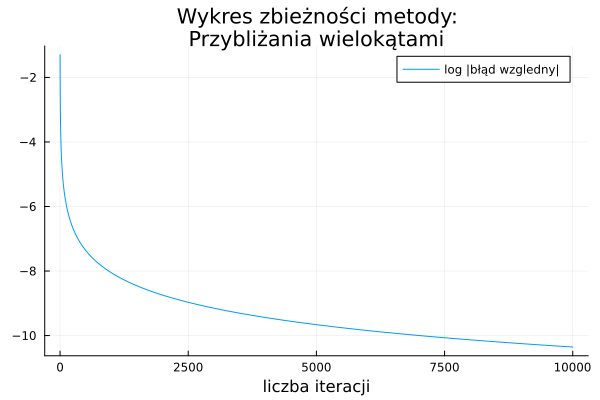
\includegraphics[width=0.6\textwidth]{../prog/geo3_log_error.png}
    \caption{Wykres ilości cyfr znaczących dla przybliżenia $\pi$ za pomocą metody geometrycznej.}
    \label{geometric-error}
\end{figure}

Zauważmy, że $\lim_{k\to\infty}L_k=2\pi$ i $\lim_{k\to\infty}l_k=2\pi$ oraz dla każdego $k$ mamy
$$l_n\leq 2\pi\leq L_n,$$
a więc możemy przybliżać $\pi$ jako
$$\pi\approx{L_n-l_n\over 4},$$
czyli jako środek przedziału $[l_n,L_n]$. Wybierzemy punkt startowy jako trójkąt równoboczny:
$$\begin{cases}
    l_3=3\sqrt3\\
    L_3=6\sqrt3
\end{cases}$$

Metoda w okolicach 8050 iteracji uzyskiwała błąd bezwzględny rzędu $10^{-12000}$. Na Wykresie~\ref{geometric-error} widzimy, że od tej iteracji, liczba dokładnie wyznaczonych cyfr osiąga granice precyzji. Jest to bardzo imponujące biorąc pod uwagę jak stara jest to metoda.

\begin{figure}[!h]\centering
    \renewcommand{\figurename}{Wykres}
    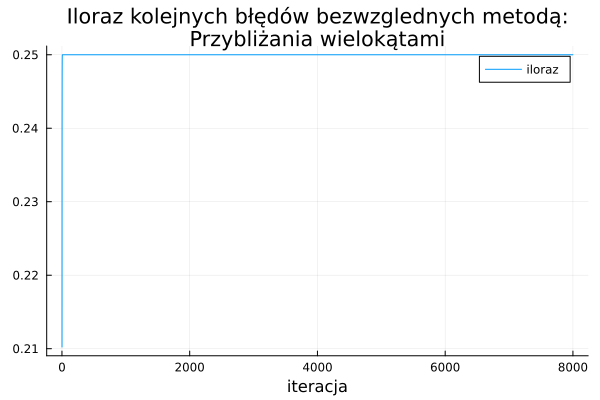
\includegraphics[width=0.7\textwidth]{../prog/geo3_error_ratio.png}
    \caption{Wykres estymowanej wartości p dla metody geometrycznej.}
    \label{geometric-convergence}
\end{figure}

Postawiliśmy hipotezę, że metoda ta jest zbieżna liniowo. Eksperymentalne wyznaczanie rzędu zbieżności potwierdziło to przypuszczenie, co widać na Wykresie~\ref{geometric-convergence}. Widać na nim, że wychodzi $p = 1$.

\subsection{Algorytm Monte Carlo}

Tak jak w poprzedniej metodzie, możemy skorzystać z faktu, że dla koła jednostkowego $\pi$ jest równe jego polu. Zauważmy, że jeżeli będziemy wybierać losowo punkty kwadratu o polu 1, to $\frac\pi4$ z nich powinno znaleźć się w ćwiartce koła o środku w jednym z wierzchołków tego kwadratu (~Rysunek \ref{fig:monte-carlo}.).

\begin{figure}[!h]\centering
\begin{tikzpicture}
    \coordinate (A) at (0,0);
    \coordinate (B) at (2,0);
    \coordinate (C) at (2,2);
    \coordinate (D) at (0,2);

    \filldraw[fill=ziel!40!white, draw=ziel] (B) arc[start angle=0, end angle=90, radius=2];
    \filldraw[color=ziel!40!white] (A)--(B)--(D)--cycle;
    \draw[thick] (A)--(B)--(C)--(D)--cycle;

    \node at (0.75, 1) {\Large$\frac\pi4$};
    \node at (1, -0.3) {\large$1$};
    \node at (-0.3, 1) {\large$1$};
\end{tikzpicture}
\caption{Stosunek pola ćwiartki koła jednostkowego do kwadratu o boku $1$}
\label{fig:monte-carlo}
\end{figure}

Korzystając z algorytmu Monte Carlo możemy wybierać losowo współrzędne $x,y\in[0,1]$ kolejnych punktów, a następnie sprawdzać ile z nich spełnia warunek
$$x^2+y^2\leq1.$$
Otrzymany stosunek będzie coraz bliższy $\frac\pi4$ wraz ze zwiększaniem ilości testowanych punktów.

Na Wykresie~\ref{monte-carlo-error}. zaprezentowana jest liczba cyfr liczby pi wyznaczonych dokładnie. Szacowanie zbieżności tej metody wykracza poza zakres wiedzy studenta 3 semestru ze względu na losowość tego algorytmu. Wykorzystanie technik z kursu Rachunku Prawdopodobieństwa ułatwiłoby to zadanie. Na Wykresie~\ref{monte-carlo-convergence} widzimy jeden z wykresów ilorazu błędu kolejnych wyrazów jaki uzyskaliśmy przy uruchamianiu algorytmu. Jako, że jest to algorytm losowy, to lokalnie wraz zwiększeniem liczby iteracji, przybliżenie może się pogorszyć. Co jest pewną wadą tej metody.

\begin{figure}[!h]\centering
\renewcommand{\figurename}{Wykres}
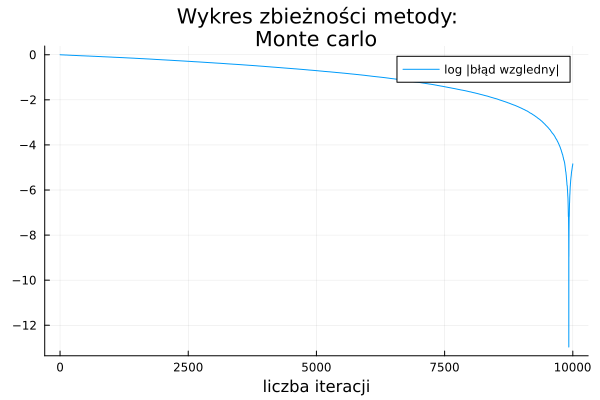
\includegraphics[width=0.6\textwidth]{../prog/monte_carlo_log_error.png}
\caption{Wykres ilości cyfr znaczących uzyskanych dla metody przybliżenia $\pi$ z pomocą algorytmu Monte Carlo.}
\label{monte-carlo-error}
\end{figure}

\begin{figure}[!h]\centering
    \renewcommand{\figurename}{Wykres}
    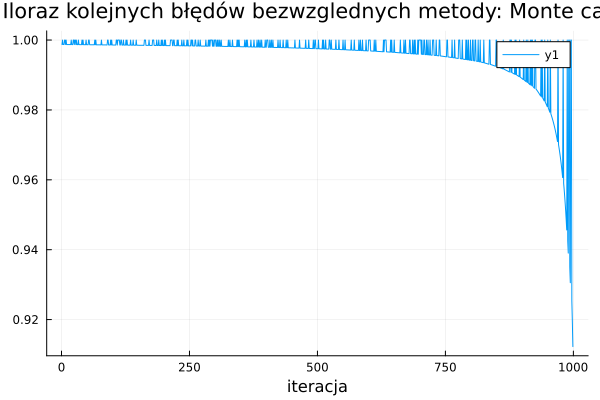
\includegraphics[width=0.6\textwidth]{../prog/monte_carlo_error_ratio.png}
    \caption{Wykres estymowanej wartości p dla metody z wykorzystaniem algorytmu Monte Carlo.}
    \label{monte-carlo-convergence}
\end{figure}


\subsection{Wielomian Taylora}
W matematyce bardzo często w celu przybliżania pożądanych wartości używa się szeregów Taylora. Tak dla przykładu, korzystając z rozszerzenia funkcji $\arctan x$ w punkcie $0$ możemy oszacować wartość $\frac\pi4$:
\begin{equation}
\begin{split}
    \frac\pi4&=\arctan1=\sum\limits_{k=0}^\infty{\arctan^{(k)}0\over k!}(1-0)^k=\\
    &=1-\frac13+\frac15-\frac17+...=\sum\limits_{k=0}^\infty{(-1)^k\over 2k+1}.
\end{split}
\end{equation}

W obliczeniach praktycznych nie możliwe jest dodawanie kolejnych elementów sumy w nieskończoność. Konieczne jest więc zatrzymanie się na pewnym $N$, co daje pewien błąd, $R_N$:
$$\frac\pi4\approx \sum\limits_{k=0}^N{(-1)^k\over 2k+1}+R_N.$$
Oznaczmy tę sumę jako $P_N$. Ponieważ dla przybliżeń funkcji wielomianem Taylora coraz wyższego stopnia dostajemy coraz dokładniejszy wynik, to $P_{N+1}$ powinno być dokładniejsze niż $P_N$. Zauważamy też, że
$$P_{N+1}-P_N={(-1)^{N+1}\over 2N+3}$$
w takim razie możemy oszacować błąd dla wielomianu Taylora $N$-tego stopnia za pomocą
$$R_N\approx \max{(-1)^{N+1}\over 2N+3}.$$

Powyższa metoda jest o wiele wolniejsza od metody Archimedesa, mimo że powstała później. W metodzie geometrycznej osiągaliśmy błąd rzędu $10^{-12000}$, natomiast wzór Taylora daje błąd rzędu $10^{-10}$. Obliczony wykładnik zbieżności tej metody wychodzi $p = 1$.

\begin{figure}[!h]\centering
    \renewcommand{\figurename}{Wykres}
    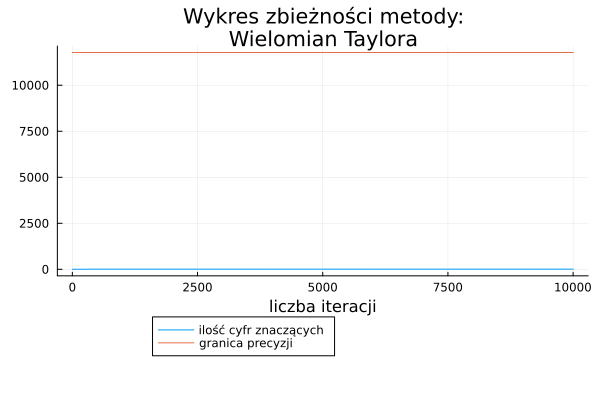
\includegraphics[width=0.7\textwidth]{../prog/taylor_log_error.png}
    \caption{Wykres ilości cyfr znaczących uzyskanych dla metody przybliżenia  $\pi$ za pomocą wielomianu Taylora.}
    \label{taylor-series-error}
\end{figure}

\begin{figure}[!h]\centering
    \renewcommand{\figurename}{Wykres}
    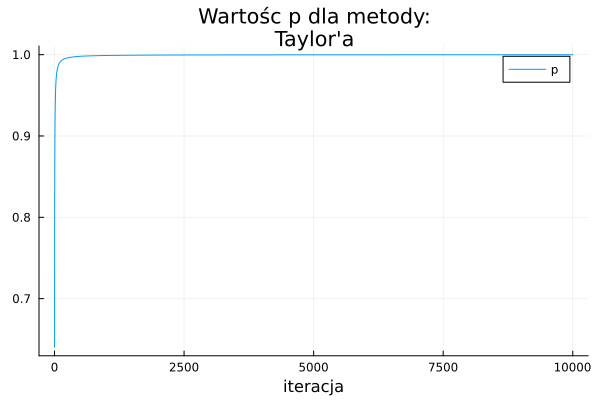
\includegraphics[width=0.7\textwidth]{../prog/taylor_error_ratio.png}
    \caption{Wykres estymowanej wartości p dla metody z wykorzystaniem wielomianu Taylora.}
    \label{taylor-series-convergence}
\end{figure}


